\documentclass{article}
\usepackage{geometry}
\geometry{hmargin = 2cm,vmargin = 2cm}
\usepackage[utf8]{inputenc}
\usepackage[T1]{fontenc}
\usepackage{amssymb}
\usepackage{amsmath}
\usepackage{amsthm}
\usepackage{mathrsfs}
\usepackage{graphicx}
\usepackage{listings} 
\usepackage{color}
\usepackage[table]{xcolor}
\definecolor{darkWhite}{rgb}{0.94,0.94,0.94}
\lstset{
  aboveskip=3mm,
  belowskip=-2mm,
  backgroundcolor=\color{darkWhite},
  basicstyle=\footnotesize,
  breakatwhitespace=false,
  breaklines=true,
  captionpos=b,
  commentstyle=\color{red},
  deletekeywords={...},
  escapeinside={\%*}{*)},
  extendedchars=true,
  framexleftmargin=16pt,
  framextopmargin=3pt,
  framexbottommargin=6pt,
  frame=tb,
  keepspaces=true,
  keywordstyle=\color{blue},
  language=python,
  literate=
  {²}{{\textsuperscript{2}}}1
  {⁴}{{\textsuperscript{4}}}1
  {⁶}{{\textsuperscript{6}}}1
  {⁸}{{\textsuperscript{8}}}1
  {€}{{\euro{}}}1
  {é}{{\'e}}1
  {è}{{\`{e}}}1
  {ê}{{\^{e}}}1
  {ë}{{\¨{e}}}1
  {É}{{\'{E}}}1
  {Ê}{{\^{E}}}1
  {û}{{\^{u}}}1
  {ù}{{\`{u}}}1
  {â}{{\^{a}}}1
  {à}{{\`{a}}}1
  {á}{{\'{a}}}1
  {ã}{{\~{a}}}1
  {Á}{{\'{A}}}1
  {Â}{{\^{A}}}1
  {Ã}{{\~{A}}}1
  {ç}{{\c{c}}}1
  {Ç}{{\c{C}}}1
  {õ}{{\~{o}}}1
  {ó}{{\'{o}}}1
  {ô}{{\^{o}}}1
  {Õ}{{\~{O}}}1
  {Ó}{{\'{O}}}1
  {Ô}{{\^{O}}}1
  {î}{{\^{i}}}1
  {Î}{{\^{I}}}1
  {í}{{\'{i}}}1
  {Í}{{\~{Í}}}1,
  morekeywords={*,...},
  numbers=left,
  numbersep=10pt,
  numberstyle=\tiny\color{black},
  rulecolor=\color{black},
  showspaces=false,
  showstringspaces=false,
  showtabs=false,
  stepnumber=1,
  stringstyle=\color{gray},
  tabsize=4,
  title=\lstname,
}
%pour la compilation minted : C:\Users\Serge\Anaconda3\pkgs\pygments-2.2.0-py37_0\Scripts à ajouter en PATH et 
%remplacer pdflatex -synctex=1 -interaction=nonstopmode %.tex
%par pdflatex -synctex=1 -interaction=nonstopmode --shell-escape %.tex
\title{2I003 : Ordonnancement d'une application sur une machine hétérogène}
\author{Arthur LIMBOUR et Serge DURAND}
\begin{document}
\maketitle
Toutes les fonctions décrites dans ce rapport sont fournis dans un fichier zip en annexe, contenant les codes sources en python.
\section{Exercice 1 : Implémentation d'un premier algorithme}

\subsection{Question 1}
\subsubsection{1 et 2 : calculs "à la main"}
Méthode : on calcule d'abord les valeurs pour les feuilles, puis pour un parent on prend le maximum de (la valeur des feuilles + l'éventuel temps de communication) et on y ajoute le temps d'exécution du parent. En effet toutes les feuilles partageant le même parent sont exécutées en même temps, donc ce qui détermine la durée d'exécution est le temps maximum parmi les feuilles + le temps de communication.\\ \\
\begin{tabular}{|c|c|c|c|c|c|c|c|c|}
  \hline
  u & 0 & 1 & 2 & 3 & 4 & 5 & 6 & 7 \\
  \hline
  $\Delta(u)$ & 13 & 7 & 1 & 7 & 2 & 3 & 5 & 7 \\
  \hline
  s(u) & 0 & 2 & 8 & 6 & 7 & 5 & 8 & 8\\
  \hline
\end{tabular}
\subsubsection{3 : Preuve de $\mathcal{P}$}
On reprend les notations de l'énoncé.
\begin{flushleft}
    \bf
    \underline{Base :}
\end{flushleft}

Soit $u \in V$ une tâche isolée, donc une arborescence réduite à un sommet, $u \in ABT(V)$. On a donc $\mathcal{G}_u = (u)$, c'est à dire $\Gamma^{+}(u) = \emptyset$ et pour une allocation donnée, la durée d'exécution minimale est simplement la durée d'exécution $t_{\sigma(u)}(u)$, donc $\mathcal{P}(u)$ est vérifiée.

\begin{flushleft}
    \bf
    \underline{Induction :}
\end{flushleft}
Soient $u \in V$ et $\Gamma^{+}(u) = \{v_{1},...,v_{p} \} \neq \emptyset$. \\
On suppose que pour tout $v$ de $\Gamma^{+}(u)$ on a $\mathcal{P}(v)$ vraie (\textbf{hypothèse d'induction}). \\
Soit $\mathcal{G}_{v_{1}},\mathcal{G}_{v_{2}},...,\mathcal{G}_{{v_p}}$ la suite d'arborescences de $ABT(V)$ telle que $\mathcal{G}_{v_i}$ est l'arborescence de durée minimale $\Delta(v_i)$ pour tout $i \in \{1,...,p\}$.\\
Alors $\forall i \in \{1,...,p\}, u \notin \mathcal{G}_{v_{i}}$, donc $\mathcal{G}_u = (u,\mathcal{G}_{v_{1}},...,\mathcal{G}_{{v_p}}) \in ABT(V)$ (par définition inductive de $ABT(V)$). \\
Toutes les tâches $v \in \Gamma^{+}(u)$ peuvent être exécutée en simultanément et donc la durée minimale d'exécution de $\mathcal{G}_u = \Delta(u)$ vaut : $max_{v \in \Gamma^{+}(u)} \{ \Delta(v) + c_{\sigma(u)\sigma(v)}((u,v))\} + t_{\sigma(u)}(u)$, car une fois la tâche $u$ effectuée il faut exécuter les tâches de chaque arborescence et l'exécution totale s'achève pour après l'exécution des tâches de l'arborescence $\mathcal{G}_{v_i}$ avec $v_i$ tel que $\Delta(v_i) + c_{\sigma(u)\sigma(v_i)}((u,v_i)) = max_{v \in \Gamma^{+}(u)} \{ \Delta(v) + c_{\sigma(u)\sigma(v)}((u,v))\}$, donc $\mathcal{P}(u)$ est vérifiée.

\begin{flushleft}
    \bf
    \underline{Conclusion :}
\end{flushleft}
On a montré que $\mathcal{P}(u)$ vraie pour toute tâche isolée $u$ puis que si $\mathcal{P}(v)$ vraie pour tout $v \in \Gamma^{+}(u)$ alors $\mathcal{P}(u)$ est vraie, donc par induction structurelle sur $ABT(V)$, la propriété est vraie pour tout $u \in V$.



\subsection{Question 2}
Pour les complexités des différentes fonctions, n est le nombre de tâches de l'arborescence étudiée, c'est aussi la longueur du tableau Arbre.
\subsubsection{Tableaux de données}
\begin{lstlisting}
Arbre = [0,0,3,0,1,1,3,3]
tA = [2,3,3,4,10,3,20,5]
tB = [3,10,1,2,2,15,5,1]
cAB = [0,1,2,4,2,3,3,3]
cBA = [0,4,3,3,4,2,3,4]
\end{lstlisting}
Note : pour les tableaux cAB et cBA on a choisit de mettre la valeur 0 pour le sommet 0, puisqu'il n'y a jamais de temps de communication pour la tâche effectuée en premier. Il n'y a aucune arête $(u,0)$ dans l'arbre.
\subsubsection{fonction duree(u,Sigmau,tA,tB)}
\begin{lstlisting}
def duree(u,Sigmau,tA,tB):
    if(Sigmau==1):
        return tA[u]
    return tB[u]
\end{lstlisting}

Complexité en $\Theta(1)$ : on fait une seule comparaison, et l'accès à un tableau est en $\Theta(1)$.

\subsubsection{fonction valCom(u,v, Sigmau,Sigmav,cAB,cBA)}
\begin{lstlisting}
def valCom(u,v,Sigmau,Sigmav,cAB,cBA):
    if(Sigmau==Sigmav):
        return 0
    elif(Sigmau==1):
        return cAB[v]
    return cBA[v]
\end{lstlisting}
Complexité en $\Theta(1)$ également, au plus 2 comparaisons, accès à cAB ou cBA en temps constant.

\subsection{Question 3 : fonction succ(u,Arbre) }
\begin{lstlisting}
def succ(u,Arbre):
    res = set()
    for i in range(1,len(Arbre)):
        if(Arbre[i] == u):
            res.add(i)
    return res
\end{lstlisting}
Complexité (en comptant le nombre de comparaison) en $\Theta(n)$ : on fait exactement n-1 comparaisons (il n'est pas nécessaire de de comparer Arbre[0] qui n'est le successeur de personne). La primitive "add" est appelée au plus (n-1) fois (cas où u = 0 et l'arbre est de hauteur 2). La complexité de "add" est en $\Theta(1)$. \\
Remarque : si on avait choisit de compter le nombre d'appels à add la complexité serait en $\mathcal{O}(n)$, mais l'instruction élémentaire de comparaison est plus significative car effectuée plus de fois que la primitive add. La primitive add étant en temps constant (comme la comparaison) son appel ne change pas la classe de complexité.
On a choisit le set plutôt que la liste pour l'utilisation dans l'exercice 2.
Par définition de nos arbres les successeurs d'un seul sommet sont uniques, le set ne pose pas de problème.
\subsection{Question 4 : CalculDelta}
On calcule la durée minimale d'exécution de $\mathcal{G}_u$ récursivement, sur le mode de la formule de la question 1 : 
le cas de base : $u$ est une tâche isolée (une feuille de l'arbre), dans ce cas la fonction renvoie $t_{\sigma(u)}(u)$. Sinon on appelle la fonction sur les successeurs de $u$. On s'est servi de la syntaxe des compréhensions de liste pour parcourir les successeurs.
\begin{lstlisting}
def CalculDelta(Arbre,tA,tB,cAB,cBA,sigma,u):
    Succ = succ(u,Arbre)
    if(len(Succ)==0):
        return duree(u,sigma[u],tA,tB)
    return duree(u,sigma[u],tA,tB) + max([CalculDelta(Arbre,tA,tB,cAB,cBA,sigma,v)+valCom(u,v,sigma[u],sigma[v],cAB,cBA) for v in Succ])
\end{lstlisting}

Complexité : 
On fait au plus $n$ appels : dans le cas où la fonction est appelée pour $u = 0$, sur la racine de l'arbre, il faut parcourir toutes les tâches de l'arborescence. 
A chaque appel récursif, (et même au premier appel) on appelle une fois la fonction succ, en $\Theta(n)$, puis si l'on est pas dans le cas de base, on fait exactement 2 additions, un appel à la primitive "max" et $k = Card(\Gamma^{+}(u))$ appels à valCom : on l'appelle sur chaque successeur de u. De plus la complexité de la primitive max est en $\Theta(k)$ puisque la taille du tableau sur laquelle elle est appelée est $k$. Finalement la complexité peut être calculée par le nombre d'appels à succ car $k \leq n$ dans tout les cas.\\
Dans le pire cas il y a n appels à succ, qui est en $\Theta(n)$. La complexité de la fonction est donc quadratique : au plus  $n*\Theta(n)$ donc $ \mathcal{O}(n^2)$.

\subsection{Question 5 : CalculSigmaOptimum}
Fonctions auxiliaires :\\
(on travaille sur les bits plutôt qu'avec les opérations arithmétiques pour tenter d'optimiser un peu... un left shift de 1 bit est par exemple une division par 2).
\begin{lstlisting}
def convBinaire(n,l):
    res =[]
    while(n!=0):
        res.append(n&1)
        n = n>>1
    res.reverse()
    #on remplit par des 0 à gauche le reste de la liste
    res = [0]*(l-len(res)) + res
    return res
    
def CalculListeAllocs(Arbre):
    n = len(Arbre)
    res = []
    for i in range(2**n-1):
        res.append(convBinaire(i,n))
    return res
    
\end{lstlisting}
Fonction principale :
\begin{lstlisting}
def CalculSigmaOptimum(Arbre,tA,tB,cAB,cBA):
    Allocs = CalculListeAllocs(Arbre)
    #Allocs = [list(tup) for tup in list(itertools.product(range(2), repeat=n))]
    Lbest = Allocs[0]
    Deltabest = CalculDelta(Arbre,tA,tB,cAB,cBA,Allocs[0],0) #vu qu'on recherche un min on peut pas initialisé à 0
    for sigma in Allocs[1:]: #pas besoin de recalculer pour la première allocation possible
        Deltatemp = CalculDelta(Arbre,tA,tB,cAB,cBA,sigma,0)
        if Deltatemp < Deltabest: #on a trouvé une meilleure allocation
            Deltabest = Deltatemp
            Lbest= sigma
    return (Lbest,Deltabest)
\end{lstlisting}

Complexité : 

Il y a $2^n$ allocations possibles. On peut le voir en remarquant que l'ensemble des allocations est en bijection avec l'ensemble des fonctions de $\{1,...,n\}$ dans $\{0,1\}$, et ce dernier ensemble à pour cardinal : $Card(\{0,1\})^{Card(\{1,...,n\})}=2^n$.
Il y a alors $2^n$ appels à CalculDelta, la complexité est donc $\Theta(n^2*2^n)$. Ici on est bien en $\Theta$ car on sait que la fonction CalculDelta est appelée d'abord sur la racine à chaque allocation. 
Note sur la constitution des allocations : nous avons testé la bibliothèque itertools pour alléger le code, mais le problème de mémoire est alors rencontré pour la même valeur de h, il n'y a pas d'améliorations notables de performance.


\section{Exercice 2 : Second Algorithme}
\subsection{Question 1}
Méthode : on calcule d'abord les deux valeurs pour chaque feuille puis on remonte l'arbre jusqu'à la racine.  \\
\\
\begin{tabular}{|c|c|c|c|c|c|c|c|c|}
  \hline
  u & 0 & 1 & 2 & 3 & 4 & 5 & 6 & 7 \\
  \hline
  $D^{\mathcal{A}}(u)$ & 13 & 7 & 3 & 12 & 10 & 3 & 20 & 5 \\
  \hline
  $D^{\mathcal{B}}(u)$ & 14 & 15 & 1 & 7 & 2 & 15 & 5 & 1 \\
  \hline
\end{tabular}
\subsection{Question 2}
On note $\mathcal{P}_2(u)$ la propriété : ($D^{\mathcal{A}}(u) \leq \Delta^{\mathcal{A}}(u)$ et $D^{\mathcal{B}}(u) \leq \Delta^{\mathcal{B}}(u)$).
\begin{flushleft}
    \bf
    \underline{Base :}
\end{flushleft}

Soit $u \in V$ une tâche isolée, donc $\mathcal{G}_u=(u)$ et $\Gamma^{+}(u) = \emptyset$.
On a alors $D^{\mathcal{A}}(u) = t_{\mathcal{A}}(u)$ et $D^{\mathcal{B}}(u) = t_{\mathcal{B}}(u)$.

On a aussi $\Delta^{\mathcal{A}}(u) = t_{\mathcal{A}}(u)$ et $\Delta^{\mathcal{B}}(u) = t_{\mathcal{B}}(u)$ puisque le seul ordonnancement réalisable possible est la simple exécution de la tâche u. Alors $D^{\mathcal{A}}(u) \leq \Delta^{\mathcal{A}}(u)$ et $D^{\mathcal{B}}(u) \leq \Delta^{\mathcal{B}}(u)$ 
\begin{flushleft}
    \bf
    \underline{Induction :}
\end{flushleft}

Soient $u \in V$ et $\Gamma^{+}(u) = \{v_{1},...,v_{p} \} \neq \emptyset$. On suppose que pour tout $v$ de $\Gamma^{+}(u)$ on a $\mathcal{P}_2(v)$ vraie (\textbf{hypothèse d'induction}). Donc, $\forall i \in \{1,...,p\}$, $D^{\mathcal{A}}(v_i) \leq \Delta^{\mathcal{A}}(v_i)$ et $D^{\mathcal{B}}(v_i) \leq \Delta^{\mathcal{B}}(v_i)$. \\
Soit $\mathcal{G}_{v_{1}},\mathcal{G}_{v_{2}},...,\mathcal{G}_{{v_p}}$ la suite d'arborescences de $ABT(V)$ telle que $\mathcal{G}_{v_i}$ est l'arborescence de durée minimale $\Delta(v_i)$ pour tout $i \in \{1,...,p\}$.\\
On note $\mathcal{G}^{\mathcal{A}}_u$ l'ordonnancement tel que $\sigma(u)=\mathcal{A}$ et $\forall v_i \in \Gamma{+}(u)$, $\mathcal{G}_{v_{i}}$ est l'ordonnancement optimal de l'arborescence avec $v_i$ en sommet. On a donc $\Delta^{\mathcal{A}}(u)$ la durée d'exécution de l'ordonnancement $\mathcal{G}^{\mathcal{A}}_u$. D'autre part $(u,\mathcal{G}_{v_{1}},...,\mathcal{G}_{{v_p}}) \in ABT(V)$ par définition inductive de $ABT(V)$. \\
Soit $k \in \{1,...,p\}$ tel que $\min(D^{\mathcal{A}}(v_k),c_{\mathcal{A}\mathcal{B}}((u,v_k)) +D^{\mathcal{B}}(v_k)) = \max\limits_{v_{i} \in \Gamma^{+}(u)} \min(D^{\mathcal{A}}(v_i),c_{\mathcal{A}\mathcal{B}}((u,v_i)) + D^{\mathcal{B}}(v_i))$. Autrement dit, $v_k$ est le fils de $u$ pour lequel l'exécution de l'ordonnancement des tâches + l'éventuel temps de communication entre $u$ et $v_k$ est la durée la plus longue parmi tout les fils de $u$ (c'est lui qui déterminera donc la durée d'exécution de $\mathcal{G}^{\mathcal{A}}_u$, puisque tout les $v_i$ peuvent être exécutée simultanément).\\
On suppose d'abord que $\min(D^{\mathcal{A}}(v_k),c_{\mathcal{A}\mathcal{B}}((u,v_k)) +D^{\mathcal{B}}(v_k)) = D^{\mathcal{A}}(v_k)$. On a donc $\sigma(v_k) = \mathcal{A}$ et : \\
$D^{\mathcal{A}}(u) = t_{\mathcal{A}}(u) + D^{\mathcal{A}}(v_k) \Rightarrow D^{\mathcal{A}}(u) \leq t_{\mathcal{A}}(u) + \Delta^{\mathcal{A}}(v_k)$ par hypothèse d'induction. \\
D'où $D^{\mathcal{A}}(u) \leq \Delta^{\mathcal{A}}(u)$. \\

Sinon on a $\min(D^{\mathcal{A}}(v_k),c_{\mathcal{A}\mathcal{B}}((u,v_k)) +D^{\mathcal{B}}(v_k)) = c_{\mathcal{A}\mathcal{B}}((u,v_k)) + D^{\mathcal{B}}(v_k)$, donc $\sigma(v_k) = \mathcal{B}$. Alors on a : \\
$D^{\mathcal{A}}(u) = t_{\mathcal{A}}(u) + c_{\mathcal{A}\mathcal{B}}((u,v_k)) + D^{\mathcal{B}}(v_k) \Rightarrow D^{\mathcal{A}}(u) \leq t_{\mathcal{A}}(u) + c_{\mathcal{A}\mathcal{B}}((u,v_k)) + \Delta^{\mathcal{B}}(v_k)$ par hypothèse d'induction, donc $D^{\mathcal{A}}(u) \leq \Delta^{\mathcal{A}}(u)$ dans les deux cas possible.

On montre de manière analogue, en considérant $\mathcal{G}^{\mathcal{B}}_u$, que dans tout les cas $D^{\mathcal{B}}(u) \leq \Delta^{\mathcal{B}}(u)$. Donc $\mathcal{P}_2(u)$ est vérifiée.

\begin{flushleft}
    \bf
    \underline{Conclusion :}
\end{flushleft}
On a montré que $\mathcal{P}_2(u)$ vraie pour toute tâche isolée $u$ puis que si $\mathcal{P}(v)$ vraie pour tout$v \in \Gamma^{+}(u)$ alors $\mathcal{P}(u)$ est vraie, donc par induction structurelle sur $ABT(V)$, la propriété est vraie pour tout $u \in V$.
\subsection{Question 3}
\subsubsection{Principe}

On commence par les feuilles et on remonte jusqu'à la racine. On fait attention à chaque étape de ne calculer des valeurs $D^{\mathcal{A}}$ et $D^{\mathcal{B}}$ uniquement pour les tâches dont ces deux valeurs sont connues \textbf{pour tout les successeurs}. Pour cela on ajoute en paramètre de la fonction un ensemble qui contient les sommets explorés (\textbf{Marques}), mis à jour à chaque appel, et un ensemble de candidats (\textbf{Candidats}) qui contient les sommets dont on veut calculer les valeurs $D^{\mathcal{A}}$ et $D^{\mathcal{B}}$. Fonctionnement :
\begin{enumerate}
\item Au premier appel on calcule les feuilles puis les valeurs $D^{\mathcal{A}}$ et $D^{\mathcal{B}}$ de chaque feuille. On insère les feuilles dans l'ensemble des candidats explorés (Marques), qui est vide pour le premier appel. On détecte que c'est le premier appel si la liste des candidats est de même taille que l'arbre. Par construction les candidats ne peuvent être l'arbre entier pour tout les appels suivants. On utilise la souplesse de python sur le typage : pour le premier appel Candidats est une liste mais pour les suivants c'est un ensemble. Les syntaxes utilisées (for u in L, ou len(Candidats)) étant applicables aux deux types.
On construit un ensemble de candidats pour le nouvel appel (Ncandidats) en y insérant les parents de chaque feuille si leurs successeurs sont tous dans l'ensemble Marques. En effet si ce n'est pas le cas il manquera des valeurs pour pouvoir calculer $D^{\mathcal{A}}$ et $D^{\mathcal{B}}$. 
\item Lors des appels suivant, si l'on est pas encore dans le dernier appel, on calcule d'abord $D^{\mathcal{A}}$ et $D^{\mathcal{B}}$ pour nos candidats, puis on les ajoute à l'ensemble des candidats explorés et on construit les nouveaux candidats comme dans le premier appel. L'ensemble des candidats explorés est conservé entre chaque appel mais celui des nouveaux candidats est mis à 0 au début de chaque appel. On sait qu'on est dans un appel intermédiaire si Candidats n'est ni l'ensemble réduit à la tâche 0, ni tout les noeuds de l'arbre.

\item Au dernier appel il ne reste plus qu'à calculer $D^{\mathcal{A}}$ et $D^{\mathcal{B}}$ pour 0, et faire un retour pour pouvoir sortir de la fonction.
\end{enumerate}
\subsubsection{Code (version commentée en annexe)}
Note : le compteur cpt n'est là que pour calculer le nombre d'appels.

\begin{lstlisting}
def CalculBorneinf(Arbre,Candidats,Marques,tA,tB,cAB,cBA,dA,dB,cpt):
    """Au premier appel Candidats = Arbre, Marques = set vide.
    dA = dB = [0]*len(Arbre)
    cpt n'est là que pour compter les appels récursifs, on le met à 0...
    """
    if(Candidats=={0}): 
        dA[0]=max([min([dA[v],dB[v]+cAB[v]]) for v in succ(0,Arbre)]) + tA[0]
        dB[0] = max([min([dB[v],dA[v]+cBA[v]]) for v in succ(0,Arbre)]) + tB[0]
        Marques.add(0).
        cpt += 1
        print(cpt)
        return (dA,dB) 
        
    NCandidats = set()
    if(len(Arbre)==len(Candidats)): 
        Candidats = Feuille(Arbre) 
        for u in Candidats:
            dA[u] = tA[u]
            dB[u] = tB[u]
            if(succ(Arbre[u],Arbre)<=Candidats): 
                NCandidats.add(Arbre[u])
        cpt += 1
        CalculBorneinf(Arbre,NCandidats,Candidats,tA,tB,cAB,cBA,dA,dB,cpt) 
    else: 
        for u in Candidats:
            dA[u] = max([min([dA[v],dB[v]+cAB[v]]) for v in succ(u,Arbre)]) + tA[u]
            dB[u] = max([min([dB[v],dA[v]+cBA[v]]) for v in succ(u,Arbre)]) + tB[u]
            Marques.add(u)          
            if(succ(Arbre[u],Arbre)<=Marques):
                NCandidats.add(Arbre[u])
        cpt += 1
        CalculBorneinf(Arbre,NCandidats,Marques,tA,tB,cAB,cBA,dA,dB,cpt)
\end{lstlisting}

Fonction auxiliaire pour le calcul des feuilles :
\begin{lstlisting}
def Feuille(Arbre):
    L = [0]*len(Arbre)
    res= set()
    for i in range(len(Arbre)):
        L[Arbre[i]] = 1           
    for i in range(len(Arbre)):
        if(L[i]==0):
            res.add(i)
            
    return res
\end{lstlisting}

\subsubsection{Complexité}
\begin{enumerate}
\item La complexité de la fonction Feuille(Arbre) est linéaire : on parcourt exactement deux fois l'arbre, et on ne fait que deux opérations maximum à chaque tour de boucle (une affectation dans une liste pour la première, une comparaison et éventuellement un ajout dans un ensemble pour la deuxième). La fonction Feuille n'est appelée qu'une fois dans la fonction CalculBorneInf.

\item On fait exactement h appels récursifs, avec h la hauteur de l'arbre. En effet on parcourt l'arbre niveau par niveau en partant des feuilles. L'arbre n'a pas de structure particulière dans les hypothèses du sujet, donc dans le pire cas on fait n appels récursif (arbre en ligne droite, chaque sommet a un seul fils).

\item Soit $k_i = Card(Candidats)$ pour le i-ème appel récursif. La primitive add et le test d'inclusion $S1 \leq S2$ (c'est la syntaxe en python) pour deux sets sont respectivement en $\Theta(1)$ et $\mathcal{O}(len(S1))$. \\
Ici aussi les $k_i$ forment une partition de $n$ (en considérant l'ensemble des feuilles et non l'arbre pour le premier appel), pour n'importe quelle structure d'arbre (par exemple si h = 2, $k_1 = n-1$ et $k_2 = 1$). \\
Pour le i-ème appel on fait $3*k_i$ appels à la fonction succ (on pourrait en faire deux en déclarant une variable Succ = succ(u)...), car on appelle 3 fois la fonction sur chaque candidat. La fonction succ étant linéaire c'est elle qui importe pour la complexité finale.
\end{enumerate}
Au final la complexité est : $(\sum\limits_{i=1}^h*k_i*3*\Theta(n)) = (\sum\limits_{i=1}^hk_i)*3*\Theta(n) = 3n*\Theta(n) = \Theta(n^2)$

\subsection{Question 4}
Ici il n'y a pas de difficulté particulière. On créé une fonction auxiliaire qui calcule l'allocation d'un sommet donné en paramètre. Elle distingue le cas où le sommet est 0. 
Puis la fonction principale appelle cette fonction auxiliaire pour tout les sommets de l'arbre grâce à un parcours en profondeur, écrit récursivement.
\subsubsection{code}
\begin{lstlisting}
def CalculSigmaOptimumAux(Arbre,tA,tB,cAB,cBA,dA,dB,Sigma,v):
    if(v==0):
        if (dA[0] <= dB[0]):
            Sigma[0]=1
        return Sigma[v]
    if(Sigma[Arbre[v]]==1):#u est dans A
        if(dA[v]<(dB[v]+cAB[v])):
            Sigma[v]=1
        else:
            Sigma[v]=0
        return Sigma[v]
    else:#u est dans B
        if(dB[v]>=(dA[v]+cBA[v])): #on inverse le test par rapport au sujet
            Sigma[v]=1
        else:
            Sigma[v]=0
        return Sigma[v]
        
def CalculSigmaOptimum2(Arbre,tA,tB,cAB,cBA,dA,dB,Sigma,Marques,u):
    """on considère sigma initialisé à 0 partout
    Marques est ici une liste de booleen : Marques[u] = 0 indique que Sigma[u] n'a pas été calculé"""
   
    Marques[u]=1
    Sigma[u] = CalculSigmaOptimumAux(Arbre,tA,tB,cAB,cBA,dA,dB,Sigma,u)
    for v in succ(u,Arbre):
        if(Marques[v]==0):
            CalculSigmaOptimum2(Arbre,tA,tB,cAB,cBA,dA,dB,Sigma,Marques,v)
\end{lstlisting}
Il suffit ensuite d'appeler cette dernière fonction pour u = 0.
\subsubsection{Complexité}
La fonction auxiliaire est en temps constant : il n'y a aucune boucle, aucune fonction auxiliaire, il n'y a qu'un nombre fini, indépendant des paramètres, d'instruction de base. \\
La fonction CalculSigmaOptimum2 fait exactement n appels récursifs grâce au suivi des sommets explorés, et à chaque appel elle invoque une fois la fonction auxiliaire et une fois la fonction succ. 
La complexité est donc quadratique. Au final pour obtenir une allocation optimale on appelle une fois CalculBorneinf et une fois CalculSigmaOptimum2 : \textbf{la complexité totale est quadratique.}

\section{Exercice 3 : mesure expérimentale de complexité}
\subsection{Question 1}
Tout est en annexe. Pour le jeu de tests l'allocation trouvée n'est pas nécessairement la même pour chaque fonction, mais dans tout les cas elle est optimale, la durée d'exécution minimale est la même. Il est en effet possible d'avoir plusieurs allocations ayant une même durée d'exécution. 
\subsection{Question 2}
Le code est laissé en annexe. On utilise la bibliothèque random et on a créé une troisième fonction qui renvoie une instance complète avec un arbre et ses données. On a écrit des fonctions pour créé des arbres droits et des arbres de hauteur 2 également. Les arbres droits servent à affiner les tests pour l'algorithme 1.
\subsection{Question 3}
Pour CalculSigmaOptimum on rencontre un problème de mémoire pour $h = 5$, c'est à dire $n = 31$. Le nombre d'opérations étant alors de l'ordre de $2^{31} = 2147483648$ opérations. En faisant des tests intermédiaires sur des arbres droits on affine : le problème de mémoire est rencontré pour n = 19. \\
On écrit une fonction qui fait le calcul d'allocation par l'algorithme 2 directement (elle appelle simplement une fois CalculBorneinf puis CalculSigmaOptimum2 en ayant initialisé des listes à 0 partout pour dA, dB etc.).
Pour cette fonction la dernière valeur de h pour laquelle l'algorithme fonctionne est h =15, donc n = 32767. A ce stade l'exécution est déjà de 2-3 minutes, il ne nous semble pas nécessaire d'affiner plus. Pour les mesures expérimentales on prendra h = 12 au plus car on répétera les tests pour une même valeur de n plusieurs fois afin de lisser les valeurs.

\subsection{Question 4}
Pour cette fonction on ne peut tester que jusqu'à h = 4 si on teste sur des arbres complets. 
Pour obtenir plus de points intermédiaires on teste sur des arbres droits jusqu'à n = 15 plutôt que sur 4 points comme suggéré par l'énoncé.

Voilà le graphe obtenu : \\
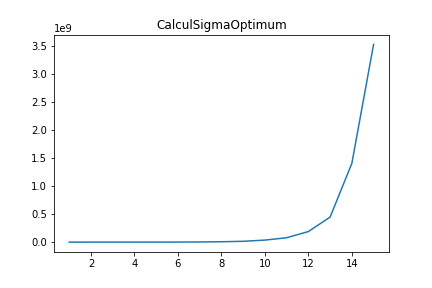
\includegraphics[scale=0.5]{CalculSigmaOptimum.png}
\\
On reconnaît la courbe d'une fonction exponentielle. Les valeurs sont ($T_1(n)$ est en ns) : \\
\begin{tabular}{|c|c|c|c|c|c|c|c|c|c|c|}
  \hline
  n & 1 & 2 & 3 & 4 & 5 & 6 & 7 & 8 & 9 & 10 \\
  \hline
  $T_1(n)$ & 8960 & 43306 & 120532 & 143786 & 379732 & 967678 & 2773116 & 6613111 & 14353475 & 36163793 \\
  \hline
\end{tabular}
\\
\begin{tabular}{|c|c|c|c|c|c|}
\hline
n &11 & 12 & 13 & 14 & 15 \\
\hline
$T_1(n)$ & 78240966 & 188379492 & 446402842 & 1404290682 & 3526867806 \\
\hline
\end{tabular} \\
En prenant le log en base 2 des $T_1(n)$ on obtient le graphe suivant : \\
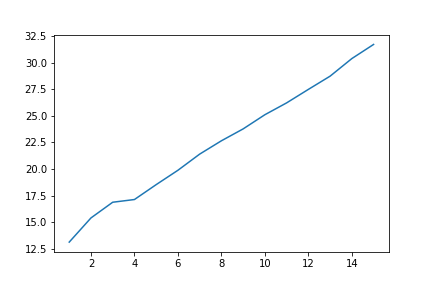
\includegraphics[scale=0.5]{Sigma1log.png} \\
La courbe est bien linéaire. On calcule sa pente en calculant la pente entre chaque points consécutifs des données obtenues et en prenant la médiane de toutes les pentes, elle vaut environ 1.33.\\
\begin{lstlisting}
def CalculPente(Lx,Ly):
    """Lx contient les abscisses (ici les tailles des arbres testés)
    Ly les ordonnées (ici le temps d'exécution)"""
    res = []
    for i in range(len(Lx)-2):
        pente = (Ly[i+1]-Ly[i])/(Lx[i+1]-Lx[i])
        res.append(pente)
    pente = np.median(res)
    return pente
\end{lstlisting}

\subsection{Question 5}

Voilà le graphe obtenu pour le test sur des hauteurs de 2 à 12, donc des tailles de 3 à 4095 : \\
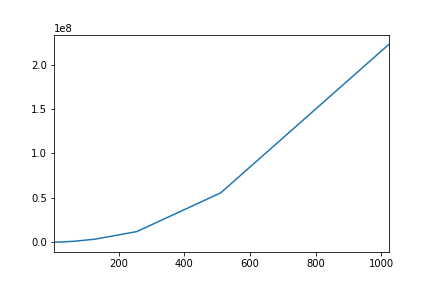
\includegraphics[scale=0.5]{CalculSigma2.png} \\
La courbe semble bien quadratique. \\
\begin{tabular}{|c|c|c|c|c|c|c|c|c|c|c|c|}
\hline
n & 3 & 7 & 15 & 31 & 63 & 127 & 255 & 511 & 1023 & 2047 & 4095 \\
\hline
$T_2(n)$ & 2 & 4.1 & 10 & 27.2 & 81.9 & 283 & 1026 & 4335 & 18011 & 72130 & 331045 \\
\hline
\end{tabular} \\
\\
Dans le tableau les valeurs de $T_2(n)$ ont été divisée par 10000 pour un tableau plus présentable.

Voilà la courbe si on divise chaque $T_2(n)$ par $n^2$ : \\
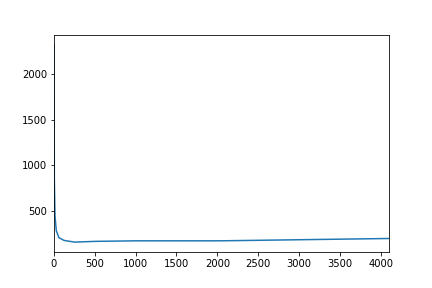
\includegraphics[scale=0.5]{CalculSigma2Normalise.png} \\
Pour des grandes valeurs de n la fonction semble bien constante, ce qui confirme que la complexité est quadratique.
\end{document}

